% ---------------------------------------------------------------------------
\subsection{Experiments}\label{sec:ngeExp}

We designed experiments to characterize the performance of the NGE on Titan,
with an emphasis on understanding its overhead and thus the cost of
introducing new functionalities. We perform three groups of experiments in
which we investigate the weak scalability, weak scalability with multiple
generation, and strong scalability of the NGE\@.

Each experiment entails executing multiple instances of AthenaMP to simulate
a pre-determined number of events. All the experiments have been performed by
configuring AthenaMP to use all the 16 cores of Titan's worker nodes.

We measured the execution time of the pilots and of AthenaMP within them,
collecting timestamps at all stages of the execution. Experiments were
performed by submitting pilots to Titan's batch queue. The turnaround time of
an individual run is determined by queue waiting times. Since we are
interested only in the performances of the NGE, we removed queue time from
our statistics.

% ---------------------------------------------------------------------------
\subsubsection{Weak scalability}

In this experiment we run as many AthenaMP instances (hereafter referred to
as tasks) as the number of nodes controlled by the pilot. Each AthenaMP
simulates 100 events, requiring \(\sim 4200\) seconds on average.

Tasks do not wait within the Agent's queue since one node is available to
each AthenaMP instance. Task execution  overheads result primarily from three
factors: (i) the initial bootstrapping of the pilot on the nodes; (ii) the
UnitManager's dispatching of units (tasks) to the agent; and (iii) time for
the Agent to bootstrap all the tasks on the nodes.

We tested pilots with 250, 500, 1000 and 2000 worker nodes and 2 hours
walltime. The time duration is determined by the Titan's walltime policy.
Fig.~\ref{fig:weakScal1a} depicts the average pilot duration, the average
execution time of AthenaMP, and the pilot overhead as function of the pilot
size.

\begin{figure}[!t]
    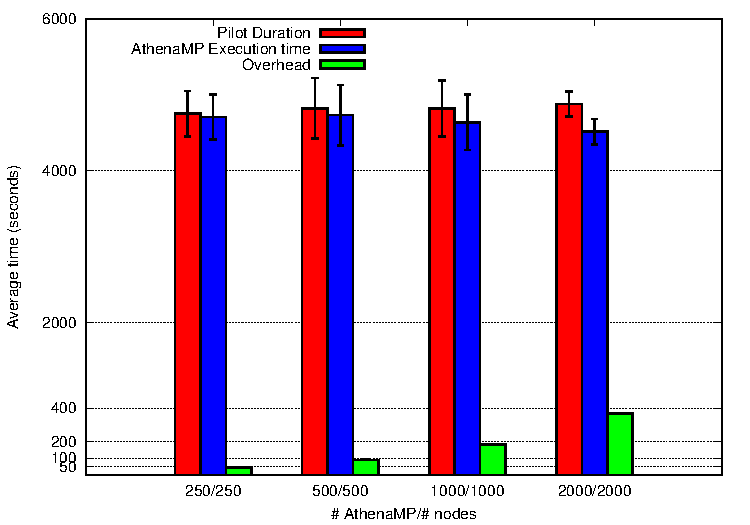
\includegraphics[height=4.5cm,width=\columnwidth]{weak1.pdf}
   	\vspace{-0.3in}
    \caption{Weak scalability: average pilot duration, average duration of
    one AthenaMP execution, and pilot's overhead as a function of pilot sizes
    (200, 500, 1000 and 2000 nodes).}\label{fig:weakScal1a}
\end{figure}

We observe that, despite some fluctuations due to external factors (e.g.,
Titan's shared filesystem and the shared database used by the NGE), the
average execution time of AthenaMP ranges between 4500 and 4800 seconds. We
also observe that in all the cases the gap between AthenaMP execution times
and the pilot durations is minimal, although it slightly increases with the
pilot size. We notice that NGE's overhead grows linearly with the number
of units.

% ---------------------------------------------------------------------------
\subsubsection{Weak scalability with multiple generation}

The NGE provides an important new capability of submitting multiple
generations of tasks to the same pilot. In order to investigate the cost
of doing so, we performed a variant of the weak scalability experiments. This
stresses the pilot's components, as new tasks are scheduled for execution on
the Agent while other tasks are still running.

In these experiments, we run five AthenaMP instances per node. As these
experiments are designed to investigate the overhead of  scheduling and
bootstraping of AthenaMP instances, the number of events simulated by each
AthenaMP task was reduced to sixteen such that the running time of each
AthenaMP was \(\approx\)1,200 seconds on average. This experiment design
choice does not affect the objectives or accuracy of the experiments, but
allows us to scale experiments to large node counts by conserving project
allocation.

We ran pilots with 256, 512, 1024 and 2048 worker nodes and 3 hours walltime.
Fig.~\ref{fig:weakScal2a} depicts the average pilot duration, the average
execution time of five generations of AthenaMP, and the corresponding
overhead. The difference between the two durations is more marked than in the
previous experiments. Despite this, we notice that the growth of the overhead
is consistent with the increment of the number of tasks per node for pilots
with 256, 512 and 1024 worker nodes, and less than linear for the pilot with
2048 worker nodes.

\begin{figure}[!t]
    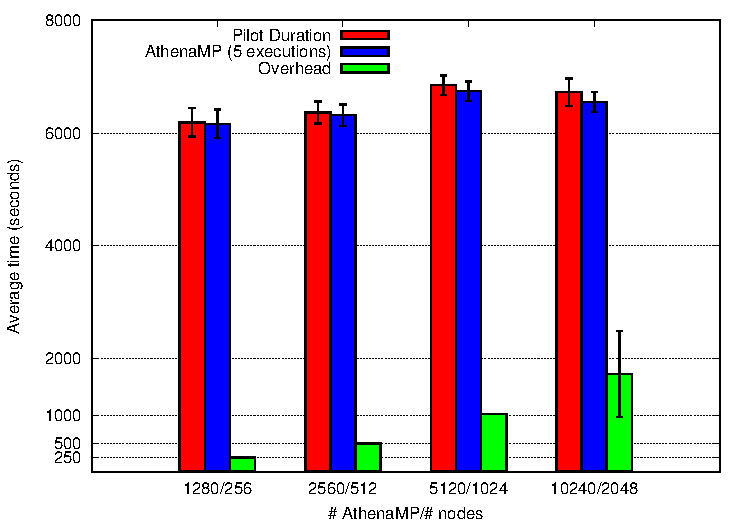
\includegraphics[height=4.5cm,width=\columnwidth]{weak2.pdf}
    \vspace{-0.3in}
    \caption{Weak scalability with multiple generations (where each
    generation has approximately 1/6th the number of events compared to Fig.
    7): average pilot duration, average duration of sequential AthenaMP
    executions, and pilot's overhead for pilot with 256, 512, 1024 and 2048
    nodes.}\label{fig:weakScal2a}
\end{figure}

%\vspace{-0.2in}

% ---------------------------------------------------------------------------
\subsubsection{Strong scalability}

We investigate strong scalability by running the same number of tasks for
different pilot sizes. We used 2048 AthenaMP instances and pilots with 256,
512, 1024 and 2048 nodes. Thus, the number of AthenaMP instances per node
(i.e., generations) is eight for the smallest pilot (256 nodes), one for the
largest pilot (2048 nodes), and with the number of generations of AthenaMP
decreasing with the pilot size. These experiments are designed to investigate
whether pilot overhead is affected by the degree of concurrency within the
pilot and/or the number of tasks. Each AthenaMP instance simulates sixteen
events as in the previous experiment.

Fig.~\ref{fig:strongScala} shows the average pilot duration and the average
execution time of possibly sequential AthenaMP instances. We notice that the
difference between the pilot duration and the AthenaMP execution times is
almost constant for all the pilot sizes, although the overall duration of the
pilot decreases linearly with the pilot size.

\begin{figure}[!t]
    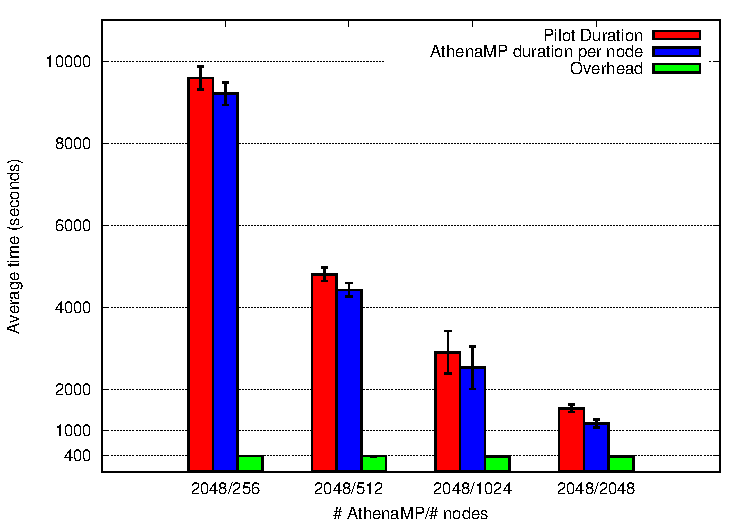
\includegraphics[height=4.5cm,width=\columnwidth]{strong.pdf}
    \vspace{-0.3in}
    \caption{Strong scalability: Average pilot duration, average duration of
    sequential AthenaMP executions, and pilot's overhead for pilots with 256,
    512, 1024 and 2048 nodes.}\label{fig:strongScala}
\end{figure}

\vspace{-0.05in}
